\section{The Arrival Problem} \label{arr}
\newcommand{\flowin}{\ensuremath{f_{\text{in}}}}
\newcommand{\glowin}{\ensuremath{g_{\text{in}}}}

The arrival problem is, given a directed graph with
a particular structure and designated source and target vertex,
decide whether or not a particular walk starting at the source
ever reaches the target. In \citep{gärtner2021subexponential} a sub-exponential
time algorithm for arrival is developed which reduces the problem to $\trsk$ of some form.
It turns out that $\arr$ is in fact polynomial time reducible to $\trsk$.
While this is not explicity stated in \citep{gärtner2021subexponential}, essentially
all of the theory for this reduction is included so credit goes to them. In this section,
I give the basic definitions of the $\arr$ problem as well as a complete proof
of polynomial time reduction from $\arr$ to $\trsk$.
\begin{definition}[Arrival Graph]
  An \emph{arrival graph} is a set of vertices $V$, a pair of
  vertices $s, t \in V$, and a pair of maps 
  $s_0, s_1 : V \to V$. 
\end{definition}
\begin{definition}[Arrival Walk]
  Let $(V, s, t, s_0, s_1)$ be an arrival graph. The \emph{arrival walk}
  on this graph is a sequence of vertices $(v_i)_{i \in \znn} \in V$
  such that $v_0 = s$, and $v_{i+1} = 
  \begin{cases} 
    s_0(v_i), & \text{$n_i$ even}\\  
    s_1(v_i), & \text{$n_i$ odd},
  \end{cases}$
  where $n_i$ is the number of times $v_i$ has appeared previously in
  the sequence.
\end{definition}
 A diagram of an example arrival graph is shown in 
in $\cref{arrivalDiagram}$.
It is clear that the arrival walk for a particular arrival graph
is entirely defined by the structure of the graph, which is what
lead it to be called a zero player graph game in \citep{arrivalBasic}.
\begin{definition}[$\textsc{Arrival}$]
  The $\textsc{Arrival}$ problem is, given an arrival graph $(V, s, t, s_0, s_1)$,
  decide whether or not the arrival walk ever reaches $t$.
\end{definition}
\begin{figure}[h]
  \centering
  \tikzset{every picture/.style={line width=0.75pt}} %set default line width to 0.75pt        

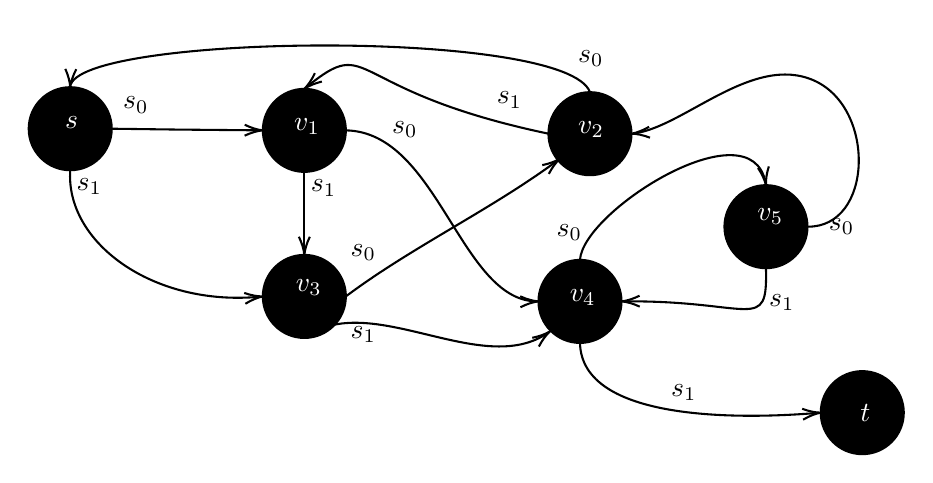
\begin{tikzpicture}[x=0.6pt,y=0.6pt,yscale=-1,xscale=1]
%uncomment if require: \path (0,300); %set diagram left start at 0, and has height of 300

%Shape: Circle [id:dp5495329281078569] 
\draw  [fill={rgb, 255:red, 0; green, 0; blue, 0 }  ,fill opacity=1 ] (32,49) .. controls (32,35.19) and (43.19,24) .. (57,24) .. controls (70.81,24) and (82,35.19) .. (82,49) .. controls (82,62.81) and (70.81,74) .. (57,74) .. controls (43.19,74) and (32,62.81) .. (32,49) -- cycle ;
%Straight Lines [id:da33331850965746734] 
\draw    (82,49) -- (121.98,49.53) -- (171,49.98) ;
\draw [shift={(173,50)}, rotate = 180.52] [color={rgb, 255:red, 0; green, 0; blue, 0 }  ][line width=0.75]    (10.93,-3.29) .. controls (6.95,-1.4) and (3.31,-0.3) .. (0,0) .. controls (3.31,0.3) and (6.95,1.4) .. (10.93,3.29)   ;
%Shape: Circle [id:dp8549825383964691] 
\draw  [fill={rgb, 255:red, 0; green, 0; blue, 0 }  ,fill opacity=1 ] (173,50) .. controls (173,36.19) and (184.19,25) .. (198,25) .. controls (211.81,25) and (223,36.19) .. (223,50) .. controls (223,63.81) and (211.81,75) .. (198,75) .. controls (184.19,75) and (173,63.81) .. (173,50) -- cycle ;
%Straight Lines [id:da15070581279870932] 
\draw    (198,75) -- (198,123) ;
\draw [shift={(198,125)}, rotate = 270] [color={rgb, 255:red, 0; green, 0; blue, 0 }  ][line width=0.75]    (10.93,-3.29) .. controls (6.95,-1.4) and (3.31,-0.3) .. (0,0) .. controls (3.31,0.3) and (6.95,1.4) .. (10.93,3.29)   ;
%Shape: Circle [id:dp4390825091110777] 
\draw  [fill={rgb, 255:red, 0; green, 0; blue, 0 }  ,fill opacity=1 ] (345,52) .. controls (345,38.19) and (356.19,27) .. (370,27) .. controls (383.81,27) and (395,38.19) .. (395,52) .. controls (395,65.81) and (383.81,77) .. (370,77) .. controls (356.19,77) and (345,65.81) .. (345,52) -- cycle ;
%Shape: Circle [id:dp9757305512769809] 
\draw  [fill={rgb, 255:red, 0; green, 0; blue, 0 }  ,fill opacity=1 ] (173,150) .. controls (173,136.19) and (184.19,125) .. (198,125) .. controls (211.81,125) and (223,136.19) .. (223,150) .. controls (223,163.81) and (211.81,175) .. (198,175) .. controls (184.19,175) and (173,163.81) .. (173,150) -- cycle ;
%Shape: Circle [id:dp6476109813645592] 
\draw  [fill={rgb, 255:red, 0; green, 0; blue, 0 }  ,fill opacity=1 ] (339,153) .. controls (339,139.19) and (350.19,128) .. (364,128) .. controls (377.81,128) and (389,139.19) .. (389,153) .. controls (389,166.81) and (377.81,178) .. (364,178) .. controls (350.19,178) and (339,166.81) .. (339,153) -- cycle ;
%Shape: Circle [id:dp9387189635111892] 
\draw  [fill={rgb, 255:red, 0; green, 0; blue, 0 }  ,fill opacity=1 ] (451,108) .. controls (451,94.19) and (462.19,83) .. (476,83) .. controls (489.81,83) and (501,94.19) .. (501,108) .. controls (501,121.81) and (489.81,133) .. (476,133) .. controls (462.19,133) and (451,121.81) .. (451,108) -- cycle ;
%Shape: Circle [id:dp6728900489022538] 
\draw  [fill={rgb, 255:red, 0; green, 0; blue, 0 }  ,fill opacity=1 ] (509,220) .. controls (509,206.19) and (520.19,195) .. (534,195) .. controls (547.81,195) and (559,206.19) .. (559,220) .. controls (559,233.81) and (547.81,245) .. (534,245) .. controls (520.19,245) and (509,233.81) .. (509,220) -- cycle ;
%Curve Lines [id:da06839655673782064] 
\draw    (223,50) .. controls (278.44,50.99) and (291.74,151.95) .. (337.6,153) ;
\draw [shift={(339,153)}, rotate = 178.78] [color={rgb, 255:red, 0; green, 0; blue, 0 }  ][line width=0.75]    (10.93,-3.29) .. controls (6.95,-1.4) and (3.31,-0.3) .. (0,0) .. controls (3.31,0.3) and (6.95,1.4) .. (10.93,3.29)   ;
%Curve Lines [id:da30024168681774177] 
\draw    (364,178) .. controls (364.99,225.52) and (461.05,224.04) .. (507.6,220.12) ;
\draw [shift={(509,220)}, rotate = 175.03] [color={rgb, 255:red, 0; green, 0; blue, 0 }  ][line width=0.75]    (10.93,-3.29) .. controls (6.95,-1.4) and (3.31,-0.3) .. (0,0) .. controls (3.31,0.3) and (6.95,1.4) .. (10.93,3.29)   ;
%Curve Lines [id:da031177664907863667] 
\draw    (370,27) .. controls (356.28,-11.22) and (69.81,-8.14) .. (57.41,22.11) ;
\draw [shift={(57,24)}, rotate = 271.79] [color={rgb, 255:red, 0; green, 0; blue, 0 }  ][line width=0.75]    (10.93,-3.29) .. controls (6.95,-1.4) and (3.31,-0.3) .. (0,0) .. controls (3.31,0.3) and (6.95,1.4) .. (10.93,3.29)   ;
%Curve Lines [id:da19551484489395188] 
\draw    (364,128) .. controls (365.79,98.44) and (466.95,34.79) .. (475.76,81.55) ;
\draw [shift={(476,83)}, rotate = 261.95] [color={rgb, 255:red, 0; green, 0; blue, 0 }  ][line width=0.75]    (10.93,-3.29) .. controls (6.95,-1.4) and (3.31,-0.3) .. (0,0) .. controls (3.31,0.3) and (6.95,1.4) .. (10.93,3.29)   ;
%Curve Lines [id:da5453571551089418] 
\draw    (345,52) .. controls (220.26,25.76) and (239.59,-8.8) .. (199.24,23.99) ;
\draw [shift={(198,25)}, rotate = 320.6] [color={rgb, 255:red, 0; green, 0; blue, 0 }  ][line width=0.75]    (10.93,-3.29) .. controls (6.95,-1.4) and (3.31,-0.3) .. (0,0) .. controls (3.31,0.3) and (6.95,1.4) .. (10.93,3.29)   ;
%Curve Lines [id:da7736997926226343] 
\draw    (223,150) .. controls (262.6,120.3) and (311.02,97.46) .. (350.8,67.9) ;
\draw [shift={(352,67)}, rotate = 143.13] [color={rgb, 255:red, 0; green, 0; blue, 0 }  ][line width=0.75]    (10.93,-3.29) .. controls (6.95,-1.4) and (3.31,-0.3) .. (0,0) .. controls (3.31,0.3) and (6.95,1.4) .. (10.93,3.29)   ;
%Curve Lines [id:da35489757719958615] 
\draw    (57,74) .. controls (54.03,117.56) and (106.93,156.22) .. (171.05,150.2) ;
\draw [shift={(173,150)}, rotate = 173.85] [color={rgb, 255:red, 0; green, 0; blue, 0 }  ][line width=0.75]    (10.93,-3.29) .. controls (6.95,-1.4) and (3.31,-0.3) .. (0,0) .. controls (3.31,0.3) and (6.95,1.4) .. (10.93,3.29)   ;
%Curve Lines [id:da7424500525745132] 
\draw    (198,175) .. controls (237.6,145.3) and (304.64,199.89) .. (344.79,171.87) ;
\draw [shift={(346,171)}, rotate = 143.13] [color={rgb, 255:red, 0; green, 0; blue, 0 }  ][line width=0.75]    (10.93,-3.29) .. controls (6.95,-1.4) and (3.31,-0.3) .. (0,0) .. controls (3.31,0.3) and (6.95,1.4) .. (10.93,3.29)   ;
%Curve Lines [id:da3132040250840804] 
\draw    (501,108) .. controls (540.44,108.6) and (542.5,36.73) .. (505,20) .. controls (468.25,3.6) and (426.87,47.76) .. (396.83,51.8) ;
\draw [shift={(395,52)}, rotate = 355.43] [color={rgb, 255:red, 0; green, 0; blue, 0 }  ][line width=0.75]    (10.93,-3.29) .. controls (6.95,-1.4) and (3.31,-0.3) .. (0,0) .. controls (3.31,0.3) and (6.95,1.4) .. (10.93,3.29)   ;
%Curve Lines [id:da9721751571878057] 
\draw    (476,133) .. controls (477,172.8) and (468.09,152.21) .. (390.18,152.99) ;
\draw [shift={(389,153)}, rotate = 359.27] [color={rgb, 255:red, 0; green, 0; blue, 0 }  ][line width=0.75]    (10.93,-3.29) .. controls (6.95,-1.4) and (3.31,-0.3) .. (0,0) .. controls (3.31,0.3) and (6.95,1.4) .. (10.93,3.29)   ;

% Text Node
\draw (87,28) node [anchor=north west][inner sep=0.75pt]   [align=left] {$\displaystyle s_{0}$};
% Text Node
\draw (52,40) node [anchor=north west][inner sep=0.75pt]  [color={rgb, 255:red, 255; green, 255; blue, 255 }  ,opacity=1 ] [align=left] {$\displaystyle s$};
% Text Node
\draw (59,77) node [anchor=north west][inner sep=0.75pt]   [align=left] {$\displaystyle s_{1}$};
% Text Node
\draw (249,43) node [anchor=north west][inner sep=0.75pt]   [align=left] {$\displaystyle s_{0}$};
% Text Node
\draw (190,41) node [anchor=north west][inner sep=0.75pt]  [color={rgb, 255:red, 255; green, 255; blue, 255 }  ,opacity=1 ] [align=left] {$\displaystyle v_{1}$};
% Text Node
\draw (200,78) node [anchor=north west][inner sep=0.75pt]   [align=left] {$\displaystyle s_{1}$};
% Text Node
\draw (361,0) node [anchor=north west][inner sep=0.75pt]   [align=left] {$\displaystyle s_{0}$};
% Text Node
\draw (361,43) node [anchor=north west][inner sep=0.75pt]  [color={rgb, 255:red, 255; green, 255; blue, 255 }  ,opacity=1 ] [align=left] {$\displaystyle v_{2}$};
% Text Node
\draw (224,117) node [anchor=north west][inner sep=0.75pt]   [align=left] {$\displaystyle s_{0}$};
% Text Node
\draw (191,138) node [anchor=north west][inner sep=0.75pt]  [color={rgb, 255:red, 255; green, 255; blue, 255 }  ,opacity=1 ] [align=left] {$\displaystyle v_{3}$};
% Text Node
\draw (224,166) node [anchor=north west][inner sep=0.75pt]   [align=left] {$\displaystyle s_{1}$};
% Text Node
\draw (348,105) node [anchor=north west][inner sep=0.75pt]   [align=left] {$\displaystyle s_{0}$};
% Text Node
\draw (356,144) node [anchor=north west][inner sep=0.75pt]  [color={rgb, 255:red, 255; green, 255; blue, 255 }  ,opacity=1 ] [align=left] {$\displaystyle v_{4}$};
% Text Node
\draw (417,201) node [anchor=north west][inner sep=0.75pt]   [align=left] {$\displaystyle s_{1}$};
% Text Node
\draw (512,101) node [anchor=north west][inner sep=0.75pt]   [align=left] {$\displaystyle s_{0}$};
% Text Node
\draw (469,95) node [anchor=north west][inner sep=0.75pt]  [color={rgb, 255:red, 255; green, 255; blue, 255 }  ,opacity=1 ] [align=left] {$\displaystyle v_{5}$};
% Text Node
\draw (476,147) node [anchor=north west][inner sep=0.75pt]   [align=left] {$\displaystyle s_{1}$};
% Text Node
\draw (531,213) node [anchor=north west][inner sep=0.75pt]  [color={rgb, 255:red, 255; green, 255; blue, 255 }  ,opacity=1 ] [align=left] {$\displaystyle t$};
% Text Node
\draw (312,25) node [anchor=north west][inner sep=0.75pt]   [align=left] {$\displaystyle s_{1}$};


\end{tikzpicture}

  \caption{The goal of the arrival problem is to decide whether a partiular walk on a directed graph with a particular
  structure reaches the target. On successive visits to a particular
  vertex the outgoing edge taken alternates. In this example
  the walk begins $s \to v_1 \to v_4 \to s \to v_3 \to \ldots$.} \label{arrivalDiagram}
\end{figure}
There is an obvious algorithm to solve the $\textsc{Arrival}$ problem;
just simulate the walk. Cases of instances where $t$ is not reachable pose a problem however -
the walk must cycle infinitely and never terminate!
The following content demonstrates that this is a non issue.
\begin{definition}[Hopeful and Desperation]
  Let $(V, s, t, s_0, s_1)$ be an instance of the $\arr$ problem. A vertex $v \in V$
  is \emph{hopeful} if there is a path $v \to t$ in the directed graph defined with
  the vertex set $V$ and edge set $E \subseteq V \times V$ with $(u, v) \in E$ if and
  only if either $s_0(u) = v$ or $s_1(u) = v$. The \emph{desperation} of a hopeful vertex
  $v$ is the length of the shortest path from $v$ to $t$.
\end{definition}
\begin{lemma}[\citep{arrivalBasic}]
  Let $(V, s, t, s_0, s_1)$  be an instance of the $\arr$ problem. If $v \in V$ is hopeful,
  the arrival walk passes through $v$ at most $2^{|V|}$ times.
\end{lemma}
\begin{proof}
  Begin by noting that if a vertex is hopeful, it's desperation is at most $|V|$. I perform
  an induction on the desperation of $v$. Suppose the desperation of $v \in V$ is 1. Then either
  $s_0(v) = t$ or $s_1(v) = t$. If $s_0(v) = t$, $t$ will be reached after passing through $v$ once.
  If $s_1(v) = t$ and $s_0(v) \neq t$ $t$ will be reached after passing through $v$ twice. In
  both cases $v$ is passed through at most $2^1 = 2$ times. \\
  Suppose that all hopeful vertices with desperation $d - 1$ are passed through at most $2^{d-1}$ times.
  Then if $v \in V$ is hopeful with desperation $d$, for some hopeful $w \in V$ with desperation
  $d - 1$ either $s_0(v) = w$ or $s_1(v) = w$. So at least every second passing of $v$, the
  walk will proceed to $w$. But the walk can pass through $w$ at most $2^{d-1}$ times,
  so the walk can pass through $v$ at most $2 \cdot 2^{d - 1} = 2^d$ times.
\end{proof}
\begin{cor}\label{walkFinite}
  Let $(V, s, t, s_0, s_1)$ be an instance of the $\arr$ problem. Then the arrival
  walk either reaches $t$, or reaches a vertex which is not hopeful.
\end{cor}
From \cref{walkFinite} it is clear that deciding an instance of the $\arr$ problem is
equivalent to deciding whether or not the arrival walk reaches $t$ or reaches a vertex which
is not hopeful.
\begin{definition}[Processed Arrival]
  Let $(V, s, t, s_0, s_1)$ be an instance of the arrival problem. It
  is without loss of generality to assume that the set of unhopeful vertices
  is non-empty. Let
  $\sim$ be the equivalence relation on $V$ generated by $u \sim v$ if
  $u$ and $v$ are both not hopeful.
  The \emph{processed arrival problem}
  is a set of vertices $V' = V / \sim$, the canonical projections of $s, t, s_0, s_1$ into $V'$,
  and a choice of representative $\overline{t} \in V'$ of all the non hopeful vertices in $V$.
\end{definition}
\begin{figure}[ht]
  \centering
  \tikzset{every picture/.style={line width=0.75pt}} %set default line width to 0.75pt        
  \raisebox{-0.5\height}{\begin{tikzpicture}[x=0.6pt,y=0.6pt,yscale=-1,xscale=1, 
  main/.style = {draw, circle, 
  fill={rgb, 255:red, 0; green, 0; blue, 0 }},
  text=white,
  node distance=2.5cm,
  ->,
  >={Stealth[round,sep]}]
  \node[main] (s) {$s$};
  \node[main] (1) [right of=s]{$v_1$};
  \node[main] (2) [right of=1]{$v_2$};
  \node[main] (3) [above right of=s]{$v_3$};
  \node[main] (4) [above right of=3]{$v_4$};
  
  % \node[main] (4) [right of=3]{$v_n$};
  \node[main] (t)[right of=3]{$t$};
  \draw (s) -- (3) node[midway, below, text=black]{$s_0$};
  \draw (s) -- (1) node[midway, below, text=black]{$s_1$};
  \draw (1) -- (2) node[midway, below, text=black]{$s_1$};
  \draw (3) -- (t) node[midway, below, text=black]{$s_1$};
  \draw (3) -- (4) node[midway, below right, text=black]{$s_0$};
  \draw (2) edge[bend left] node[near start, above, text=black]{$s_0$} (1);
  \draw (1) edge[bend left] node[near start, below, text=black]{$s_0$}(2);

  \draw (4.south) to[bend left=120, min distance=1.6cm] node[midway, left, text=black]{$s_0$} (4.north);
  \draw (4.south) to[bend left=120, min distance=2.4cm] node[midway, left, text=black]{$s_1$} (4.north);
  % \draw (4) edge[bend left] node[near start, above, text=black]{$s_0$}(1);
  \draw (2) edge[bend right=70, min distance=0.8cm] node[near start, below, text=black]{$s_1$} (1.south);
\end{tikzpicture}
}
  \hfil
  $\mapsto$
  \hfil
  \raisebox{-0.5\height}{\begin{tikzpicture}[x=0.6pt,y=0.6pt,yscale=-1,xscale=1, 
  main/.style = {draw, circle, 
  fill={rgb, 255:red, 0; green, 0; blue, 0 }},
  text=white,
  node distance=2.5cm,
  ->,
  >={Stealth[round,sep]}]
  \node[main] (s) {$s$};
  \node[main] (1) [right of=s]{$\overline{t}$};
  \node[main] (3) [above right of=s]{$v_3$};
  
  % \node[main] (4) [right of=3]{$v_n$};
  \node[main] (4)[right of=3]{$t$};
  \draw (s) -- (3) node[midway, below, text=black]{$s_0$};
  \draw (s) -- (1) node[midway, below, text=black]{$s_1$};
  \draw (3) -- (4) node[midway, below, text=black]{$s_1$};
  \draw (3) -- (1) node[midway, above right, text=black]{$s_0$};
\end{tikzpicture}
}
  \caption{Instances of the arrival problem can be preprocessed so that every non-target vertex
  has a directed path to the target. An extra 'bad target' $\overline{t}$ is added which represents
  all the vertices with no directed path to the target $t$, and the problem becomes to decide
  which of the two targets is reached. From \cref{walkFinite} 
  the walk in the resultant graph must be finite.}\label{arrivalPreprocess}
\end{figure}
Noting that the set of non hopeful vertices can be easily computed in linear time with a breadth first search
from $t$, from this point on I will refer
to instances of the $\arr$ problem exclusively as tuples $(V, s, t, \overline{t}, s_0, s_1)$ 
constructed as above.
\begin{cor}[\citep{arrivalBasic}]
  The time complexity of the $\arr$ problem is $O(n \cdot 2^n)$.
\end{cor}
\begin{proof}
  I reason that the arrival walk on the processed instance $(V, s, t, \overline{t}, s_0, s_1)$
  has it's walk length bounded by $O(n \cdot 2^n)$. Every vertex $v \in V$ with $v \neq \overline{t}$
  is hopeful with desperation at most $n$, so by \cref{walkFinite} can be passed through at most
  $2^{n}$ times. If the walk reaches $t$ or $\overline{t}$ it terminates, and there are at most
  $n$ vertices $w \in V$ such that $w \not\in \{t, \overline{t}\}$, so the walk can take at most
  $n \cdot 2^n$ steps.
\end{proof}
There are in fact instances of the $\arr$ problem with exponentially long walks -
as seen in \cref{expLongArrival} - implying that the worst-case runtime of this algorithm is exponential.
Recently a sub-exponential\footnote{Specifically an algorithm running
in time $O(2^{\sqrt{n}})$.} upper bound for $\arr$ was given in \citep{gärtner2021subexponential}.
Interestingly, their algorithm involves a reduction from $\arr$ to $\trsk$. I will not detail
the reduction used in the sub-exponential algorithm, but will spend the remainder of the section
demonstrating a similar, yet simpler reduction from $\arr$ to $\trsk$.
\begin{figure}[h]
  \centering
  \tikzset{every picture/.style={line width=0.75pt}} %set default line width to 0.75pt        

\begin{tikzpicture}[x=0.6pt,y=0.6pt,yscale=-1,xscale=1, 
  main/.style = {draw, circle, 
  fill={rgb, 255:red, 0; green, 0; blue, 0 }},
  text=white,
  node distance=3cm,
  ->,
  >={Stealth[round,sep]}]
  \node[main] (1) {$s$};
  \node[main] (2) [right of=1]{$v_1$};
  \node[main] (3) [right of=2]{$v_2$};
  \node[main] (4) [right of=3]{$v_n$};
  \node[main] (5)[right of=4]{$t$};
  \node[text=black] at ($(3)!.5!(4)$) {\ldots};
  \draw (1) -- (2) node[midway, below, text=black]{$s_1$};
  \draw (2) -- (3) node[midway, below, text=black]{$s_1$};
  \draw (4) -- (5) node[midway, below, text=black]{$s_1$};
  % \path (1) edge[loop above] node {$s_0$} (1);
  \draw (2) edge[bend left] node[near start, above, text=black]{$s_0$} (1);
  \draw (3) edge[bend left] node[near start, above, text=black]{$s_0$}(1);
  \draw (4) edge[bend left] node[near start, above, text=black]{$s_0$}(1);
\end{tikzpicture}

  \caption{There are instances of the arrival problem with exponentially long walks. An induction
  on the number of steps to get from $s \to v_i$ shows that walk on the above
  takes at least $\Omega(2^n)$ steps to reach $t$.}\label{expLongArrival}
\end{figure}
\begin{definition}[Switching Flow]
  Let $(V, s, t, \overline{t}, s_0, s_1)$ be an arrival graph. A \emph{switching flow} is a pair of maps 
  $f_0, f_1 : V \setminus \{t, \overline{t}\} \to \znn$ such that the following axioms hold.
    Let $\flowin(v) =
        \sum_{\substack{w \in V \\ s_0(w) = v}} f_0(w) 
        + \sum_{\substack{w \in V \\ s_1(w) = v}} f_1(w)$. 
  \begin{itemize}
    \item For all $v \in V \setminus \{s, t, \overline{t}\}$, $\flowin(v) = f_0(v) + f_1(v)$ (flow conservation),
    \item $\flowin(s) = f_0(s) + f_1(s) - 1$ (source flow conservation),
    \item For all $v \in V$, $f_1(v) \leq f_0(v) \leq f_1(v) + 1$ (switching).
  \end{itemize}
\end{definition}
\begin{notation}
  Throughout this section if $a \in \znn^d$ and $(f_0, f_1)$ is the flow
  corresponding to $a$, the notation $\flowin(v) =
        \sum_{\substack{w \in V \\ s_0(w) = v}} f_0(w) 
        + \sum_{\substack{w \in V \\ s_1(w) = v}} f_1(w)$ will be used. 
\end{notation}
  It was observed in \citep{arrivalBasic} that the walk on an arrival graph can be characterized
  by a switching flow.
  \begin{lemma}[\citep{arrivalBasic}]\label{walkSwitching}
    Let $(V, s, t, \overline{t}, s_0, s_1)$ be an instance of the $\arr$ problem. Define
    $f_0 : V \setminus \{t, \overline{t}\} \to \znn$ by $f_0(v) =$ the number of times $s_0(v)$
    is traversed in the arrival walk, and define $f_1$ similarly. Then $(f_0, f_1)$ is a switching
    flow.
  \end{lemma}
  \begin{proof}
    Flow conservation and source flow conservation follow from the fact that the walk must walk
    out of a vertex if it walks in, minus the initial step it takes from the source. Switching
    follows from the nature of the walk taking the $s_0$ edge on even passes, and $s_1$ edge on odd
    passes.
  \end{proof}
  I next establish a correspondence from arrival instances to monotone functions.
  \begin{definition}[Arrival Monotone Function]
    Let $(V, s, t, \overline{t}, s_0, s_1)$ be an instance of the arrival problem,
    $d = |V \setminus \{t, \overline{t}\}|$ and
    $(v_i)_{i \in [d]}$ be an enumeration of the vertices in 
    $V \setminus \{t, \overline{t}\}$. The \emph{arrival monotone function} is a function
    $f : \znn^d \to \znn^d$ defined coordinatewise as,
  \begin{align*}
    f((a_1, ..., a_d))_i = \begin{cases}
    \sum_{\substack{j \in [d] \\ s_0(v_j) = v_i}} \left\lceil \frac{a_j}{2} \right\rceil
      + \sum_{\substack{j \in [d] \\ s_1(v_j) = v_i}} \left\lfloor \frac{a_j}{2} \right\rfloor
      & v_i \neq s \\
    1 + \sum_{\substack{j \in [d] \\ s_0(v_j) = v_i}} \left\lceil \frac{a_j}{2} \right\rceil
      + \sum_{\substack{j \in [d] \\ s_1(v_j) = v_i}} \left\lfloor \frac{a_j}{2} \right\rfloor
      & v_i = s.
    \end{cases}
  \end{align*}
  \end{definition}
  \begin{lemma}\label{arrMonotoneIsMonotone}
    The arrival monotone function is monotone.
  \end{lemma}
  \begin{proof}
    Clearly the sum of monotone functions is also monotone, $\lceil \cdot \rceil$ and $\lfloor \cdot \rfloor$
    are monotone, composition of monotone functions is monotone, linear functions with non-negative coefficients
    are monotone, and constant functions are monotone. This encompasses all components of the above function,
    which is therefore montone.
  \end{proof}
  The monotone function was constructed precisely so that the following proposition holds.
  \begin{prop}\label{fixpointIsFlow}
    Let $f : \znn^d \to \znn^d$ be an arrival monotone function, and $a = (a_1, ..., a_d) \in \znn^d$. 
    Define $g_0(v_i) = \lceil \frac{a_i}{2} \rceil$ and $g_1(v_i) = \lfloor \frac{a_i}{2} \rfloor$. 
    If $f(a) = a$ then $(g_0, g_1)$ is a switching flow.
  \end{prop}
  \begin{proof}
    For flow conservation, let $v_i \in V \setminus \{s, t, \overline{t}\}$. Then,
    \begin{align*}
      \sum_{\substack{j \in [d] \\ s_0(v_j) = v_i}} g_0(v_j) 
      + \sum_{\substack{j \in [d] \\ s_0(v_j) = v_i}} g_1(v_j) &= 
      \sum_{\substack{j \in [d] \\ s_0(v_j) = v_i}}  \left\lceil \frac{a_j}{2} \right\rceil
      + \sum_{\substack{j \in [d] \\ s_0(v_j) = v_i}} \left\lfloor \frac{a_j}{2} \right\rfloor \\
      &= f(a)_i \\ 
      &= a_i \\ 
      &= \left\lceil \frac{a_i}{2}\right\rceil + \left\lfloor \frac{a_i}{2}\right\rfloor \\
      &= g_0(v_i) + g_1(v_1).
    \end{align*}
    Source flow conservation follows similarly. Switching is clear from the definition of $\lfloor \cdot \rfloor$
    and $\lceil \cdot \rceil$. \\
  \end{proof}
  The next proposition draws useful connection between the arrival walk and monotone function.
  \newcommand{\lc}{\left\lceil}
  \newcommand{\rc}{\right\rceil}
  \newcommand{\lf}{\left\lfloor}
  \newcommand{\rf}{\right\rfloor}
  \begin{prop}\label{kleeneTarskiIsWalk}
    Let $(V, s, t, \overline{t}, s_0, s_1)$ be an instance of the problem, and $f$ be the 
    arrival monotone function. For $a \in \znn^d$ let $g_0(a) = \lc \frac{a}{2} \rc$ and 
    $g_1(a) = \lf \frac{a}{2} \rf$. For $i \in \{x \in \znn | x < n \}$ where $n$ number of steps
    to reach $t$ or $\overline{t}$, let 
    $(h_0^i : [d] \to \znn, h_1a^i : [d] \to \znn)_{i \in \znn}$
    be a sequence defined by $h_0^i(j) = $ the number of times the $s_0$ edge has been taken from $v_j$
    after $i$ steps in the walk, and define $h_1^i(j)$ similarly for the $s_1$ edge. Then for each $j \in [d]$
    $g_0(f^i(\vec{0}))_j = h_0^i(j)$ and $g_1(f^i(\vec{0}))_j = h_1^i(j)$.
  \end{prop}
  \begin{proof}
    By induction. For the base case where $i = 0$ no edges have been crossed, so for each
    $j \in [d]$ $h_0^i(j) = h_1^i(j) = 0 = \frac{f^0(\vec{0})_i}{2} = 0$. \\
    So suppose for some $i \in \znn$ the statement is true for all $j \in [i-1]$.
    Let $v_k \in V \setminus \{t, \overline{t}\}$ be the vertex the walk is at after $i - 1$ steps, and $v_l$ after $i-2$ steps.
    Then by the inductive hypothesis $f^{i-2}(\vec{0})_l + 1 = f^{i-1}(\vec{0})_l$ and for each
    $m \in [d] \setminus \{l\}$, $f^{i-2}(\vec{0})_m = f^{i-1}(\vec{0})_m$. It follows that
    $f^{i - 1}(\vec{0})_k + 1 = f^{i}(\vec{0})_k$, and the switching property of the monotone function
    guarantees that the extra unit appears on the correct edge.
  \end{proof}
  All of that is really just to say that in the case of monotone functions from the arrival problem,
  \emph{iteration from the bottom of the lattice as in \cref{kleeneTarski} is the walk}. This connection gives
  me some useful corollaries.
  \begin{cor}\label{walkLfp}
    Let $f$ be an arrival monotone function, 
    $(g_0, g_1)$ be the switching flow corresponding to an arrival walk as in \cref{walkSwitching},
    and $a \in \znn^d$ be the fixpoint corresponding to this switching flow as in \cref{fixpointIsFlow}.
    Then $a$ is the least fixpoint of $f$.
  \end{cor}
  \begin{proof}
    Using a similar argument to \cref{kleeneLfp}, iteration from the bottom of the lattice gives the least
    fixpoint. But \cref{kleeneTarskiIsWalk} says that iteration from the bottom of the lattice is the walk
    and will give the fixpoint corresponding to the switching flow of the walk.
  \end{proof}
  \begin{lemma} \label{flowSunk}
    Let $f : \znn^d \to \znn^d$ be an arrival monotone function. If $a \in \znn^d$ and
    $(f_0, f_1)$ the flow corresponding to $a$, then 
    $\sum_{i \in [d]} f(a)_i =  1 + \left( \sum_{i \in [d]} a_i \right) - \flowin(t) - \flowin(\overline{t})$.
  \end{lemma}
  \begin{proof}
    Easily computed from the definitions.
  \end{proof}
  \begin{cor}
    Let $A$ be an instance of the arrival problem and $(g_0, g_1)$ a switching flow.
    Then either $\glowin (t) = 1$ and $\glowin (\overline{t}) = 0$,
    or $\glowin (t) = 0$ and $\glowin (\overline{t}) = 1$.
  \end{cor}
  \begin{proof}
    The walk only terminates when it reaches either $t$ or $\overline{t}$, so if $(f_0, f_1)$ 
    is the switching flow corresponding
    I must have exactly one of $\flowin(t) = 1$ and $\flowin(\overline{t}) = 0$ or 
    $\flowin(t) = 0$ and $\flowin(\overline{t}) = 1$. By \cref{walkLfp} the walk corresponds
    to the least fixpoint, and for all other switching flows $(g_0, g_1)$, at least one of $\glowin (t) \geq 1$ or
    $\glowin (\overline{t}) \geq 1$. Suppose for a contradiction that $\glowin (t) + \glowin (\overline{t}) \geq 2$ and let
    $a \in \znn^d$ be the point corresponding to $(g_0, g_1)$. If $f$ is the arrival monotone function corresponding to $A$ then by \cref{flowSunk},
      $\sum_{i \in [d]} f(a)_i = 1 + \left( \sum_{i \in [d]} a_i\right) 
        - \glowin(t) - \glowin(\overline{t})
                              \leq \sum_{i \in [d]} a_i - 1$.
    Which contradicts $a$ being a fixpoint and $(g_0, g_1)$ being a switching flow.
  \end{proof}
  Remarkably, this implies that \emph{any} switching flow is certificate to the walk reaching either $t$
  or $\overline{t}$. Further, fixpoints are switching flows so deciding the $\arr$ problem is reducible
  to finding a fixpoint of a particular monotone function! I'm not quite finished yet however;
  the monotone functions of arrival instances considered so far have been on the infinite lattice $\znn^d$, but
  the $\trsk$ problem I defined is on the finite lattice $[N]^d$. This will turn out to not be an issue.
  \begin{notation}
    For $N \in \znn$ notation $[N]_0$ represents $[N] \cup \{0\}$.
  \end{notation}
  \newcommand{\no}{[N]_0}
  \begin{definition}[Bounded arrival monotone function]
    Let $(V, s, t, \overline{t}, s_0, s_1)$ be an instance of the arrival problem and $f$
    be it's corresponding arrival function. Let $n = |V|$ and $N = 2^n$. The \emph{bounded arrival monotone function}
    is a function $F : \no^d \to \no^d$ defined coordinatewise as $F(a)_i = \min(f(a)_i, N)$. 
  \end{definition}
  \begin{lemma}
    Let $F$ be a bounded arrival monotone function. Then $F$ is monotone.
  \end{lemma}
  \begin{proof}
    Similarly to the proof of \cref{arrMonotoneIsMonotone}, $\min(\cdot, \; N)$ is clearly monotone.
    Monotonicity then follows monotonicity of the arrival monotone function, and monotonicity
    being preserved under composition.
  \end{proof}
  \begin{lemma}[\citep{gärtner2021subexponential}]
    Let $(V, s, t, \overline{t}, s_0, s_1)$ be an instance of the arrival problem, 
    $n = |V|$, $N = 2^n$, $d = |V \setminus \{t, \overline{t}\}|$, 
    $f : \znn^d \to \znn^d$ be the arrival monotone function, and $F : \no^d \to \no^d$
    be the bounded arrival monotone function.
    If $a \in \no^d$ satisfies $F(a) = a$, then $f(a) = a$. 
  \end{lemma}
  \begin{proof}
    Begin by noting that for all $a \in \no^d$, $f(a) \geq F(a)$. Suppose for a contradiction that $f(a) \neq F(a)$.
    Then $F(a) > f(a)$. From \cref{flowSunk},
    $\sum_{i \in [d]} f(a)_i \leq 1 + \sum_{i \in [d]} a_i$. 
    Since $F(a) = a$ I find $i \in [d]$, $f(a)_j = 
    \begin{cases} a_j + 1 & j = i \\ a_j & j \neq i. \end{cases}$. By definition $F(a)_i = \min(f(a)_i, N)$
      so $a_i = N$ and $f(a)_i = N + 1$.
    For $\sum_{i \in [d]} f(a)_i = 1 + \sum_{i \in [d]} a_i$ 
    I require that $f_{\text{in}}(t) = 0$ and $f_{\text{in}}(\overline{t}) = 0$.
    But \cref{walkFinite} combined with $a_i = N = 2^n$ implies that the walk must have terminated. That is,
    either $f_{\text{in}}(t) > 0$ or $f_{\text{in}}(\overline{t}) > 0$, which is a contradiction. 
  \end{proof}
  \begin{theorem}
    $\arr$ is polynomial time reducible to $\trsk$.
  \end{theorem}
